% tugas_data_analitik.tex
% Laporan Tugas Data Analitik — C-MAPSS RUL Prediction
% Departemen Teknik Mesin FTUI — 2026

\documentclass[11pt,a4paper]{article}

% ── Packages ──────────────────────────────────────────────────────────────────
\usepackage[T1]{fontenc}
\usepackage[utf8]{inputenc}
\usepackage[a4paper, margin=2.5cm]{geometry}


\usepackage{setspace}
\usepackage{parskip}
\usepackage{titlesec}
\usepackage{fancyhdr}
\usepackage{booktabs}
\usepackage{tabularx}
\usepackage{multirow}
\usepackage{longtable}
\usepackage{graphicx}
\usepackage{caption}
\usepackage{subcaption}
\usepackage{xcolor}
\usepackage{amsmath}
\usepackage{hyperref}
\usepackage{enumitem}
\usepackage{float}

% ── Colors ────────────────────────────────────────────────────────────────────
\definecolor{uiblue}{RGB}{0,56,147}
\definecolor{mygray}{RGB}{100,100,100}
\definecolor{lightgray}{RGB}{240,240,240}

% ── Section formatting ────────────────────────────────────────────────────────
\titleformat{\section}
  {\large\bfseries\color{uiblue}}
  {\thesection}{0.6em}{}[\vspace{2pt}\hrule\vspace{4pt}]

\titleformat{\subsection}
  {\normalsize\bfseries\color{uiblue}}
  {\thesubsection}{0.6em}{}

\titleformat{\subsubsection}
  {\small\bfseries}
  {\thesubsubsection}{0.6em}{}

% ── Header / Footer ───────────────────────────────────────────────────────────
\pagestyle{fancy}
\fancyhf{}
\fancyhead[L]{\small\color{mygray}
  Tugas Data Analitik -- Prediksi RUL Mesin Turbofan C-MAPSS}
\fancyhead[R]{\small\color{mygray} Departemen Teknik Mesin FTUI}
\fancyfoot[C]{\small\color{mygray}\thepage}
\renewcommand{\headrulewidth}{0.4pt}
\renewcommand{\footrulewidth}{0.0pt}

\onehalfspacing
\captionsetup{font=small, labelfont=bf}

% ── Hyperref ──────────────────────────────────────────────────────────────────
\hypersetup{
  colorlinks=true,
  linkcolor=uiblue,
  urlcolor=uiblue,
  citecolor=uiblue,
}

% ══════════════════════════════════════════════════════════════════════════════
\begin{document}

% ── Cover Page ────────────────────────────────────────────────────────────────
\begin{titlepage}
  \centering
  \vspace*{1.0cm}

  
\includegraphics[width=2.2cm]{images/logo_ui.png}

  \vspace{0.6cm}
  {\large\bfseries UNIVERSITAS INDONESIA\par}
  \vspace{0.2cm}
  {\normalsize Fakultas Teknik -- Departemen Teknik Mesin\par}

  \vspace{0.5cm}
  \hrule height 1.2pt
  \vspace{0.4cm}
  {\LARGE\bfseries\color{uiblue}
    PREDIKSI \textit{REMAINING USEFUL LIFE}\\[0.3em]
    MESIN TURBOFAN MENGGUNAKAN\\[0.3em]
    \textit{ARTIFICIAL NEURAL NETWORK}\\[0.3em]
    PADA DATASET C-MAPSS\par}
  \vspace{0.4cm}
  \hrule height 1.2pt

  \vspace{1.0cm}
  {\normalsize\color{mygray} Mata Kuliah:\par}
  {\large\bfseries Data Analitik\par}

  \vspace{0.6cm}
  {\normalsize\color{mygray} Dosen Pengampu:\par}
  {\normalsize Dr.\ Eng.\ Sholahudin, S.T., M.Sc.\par}

  \vspace{0.8cm}
  {\normalsize\color{mygray} Disusun Oleh:\par}
  \vspace{0.4cm}
  \begin{tabular}{ll}
    2506565466 & Luqman Alifio Arhab \\[4pt]
    2506565414 & Azfa Rhazasta Abiandra \\[4pt]
    2506565401 & Adamsyah Haryo Saksono \\[4pt]
    2506565433 & Epsiarto Rizqi Nurwijayadi \\[4pt]
  \end{tabular}

  \vspace{0.2cm}
  \vfill
  {\normalsize\bfseries
    DEPARTEMEN TEKNIK MESIN\\
    FAKULTAS TEKNIK\\
    UNIVERSITAS INDONESIA\\[0.4em]
    2026\par}
\end{titlepage}

\thispagestyle{empty}
\newpage
\setcounter{page}{1}

% ══════════════════════════════════════════════════════════════════════════════
\section{Pendahuluan}

Prediksi \textit{Remaining Useful Life} (RUL) merupakan komponen penting dalam
\textit{prognostics and health management} (PHM) sistem mekanik. Dengan mengetahui
sisa umur pakai suatu komponen, jadwal perawatan dapat dioptimalkan sehingga
mengurangi biaya \textit{downtime} dan risiko kegagalan mendadak.

Laporan ini mendokumentasikan pipeline analitik lengkap untuk memprediksi RUL
mesin turbofan menggunakan dataset C-MAPSS (\textit{Commercial Modular Aero-Propulsion
System Simulation}) dari NASA \cite{saxena2008}. Pipeline mencakup pembersihan data,
normalisasi, seleksi fitur dengan \textit{Principal Component Analysis} (PCA) dan
korelasi Pearson, pemodelan dengan \textit{Multilayer Perceptron} (MLP), serta
analisis kepentingan fitur dengan algoritma Garson.

\begin{figure}[H]
  \centering
  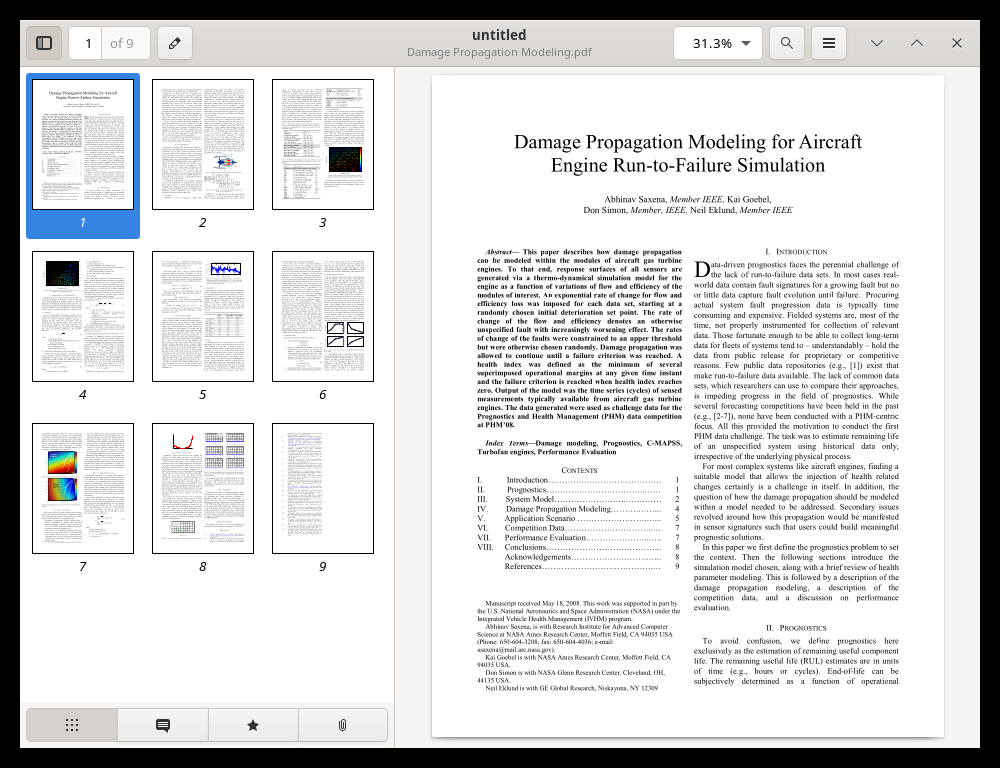
\includegraphics[width=0.55\textwidth]{images/data-source-01-paper.png}
  \caption{Dataset C-MAPSS --- makalah referensi (Saxena et al., PHM08)}
  \label{fig:paper}
\end{figure}

% ══════════════════════════════════════════════════════════════════════════════
\section{Dataset C-MAPSS}

\subsection{Deskripsi Dataset}

Dataset C-MAPSS terdiri dari empat sub-dataset dengan karakteristik yang berbeda,
memungkinkan evaluasi model pada tingkat kompleksitas yang bervariasi.

\begin{table}[H]
\centering
\small
\caption{Karakteristik empat sub-dataset C-MAPSS}
\label{tab:dataset}
\begin{tabular}{lcccccc}
\toprule
Sub-dataset & Kondisi & Mode Kerusakan &
  \multicolumn{2}{c}{Jumlah Mesin} &
  \multicolumn{2}{c}{Jumlah Baris} \\
\cmidrule(lr){4-5}\cmidrule(lr){6-7}
& Operasi & & Train & Test & Train & Test \\
\midrule
FD001 & 1 & HPC         & 100 & 100 & 20.631 & 13.096 \\
FD002 & 6 & HPC         & 260 & 259 & 53.759 & 33.991 \\
FD003 & 1 & HPC + Fan   & 100 & 100 & 24.720 & 16.596 \\
FD004 & 6 & HPC + Fan   & 248 & 248 & 61.249 & 41.214 \\
\bottomrule
\end{tabular}
\end{table}

Setiap baris data terdiri dari 26 kolom: \texttt{unit\_number}, \texttt{time\_cycles},
tiga \textit{operational settings}, dan 21 sensor. Data \textit{train} mencatat siklus
penuh hingga kegagalan; data \textit{test} dipotong sebelum kegagalan. File
\texttt{RUL\_FDxxx.txt} berisi RUL sebenarnya pada titik pemotongan sebagai kunci
jawaban evaluasi.

\subsection{Struktur HDF5}

Seluruh data disimpan dalam format HDF5 menggunakan satu skrip konsolidasi
\texttt{build\_cmapss\_complete.py} yang membaca langsung dari file \texttt{.txt}
NASA tanpa file perantara.

\begin{figure}[H]
  \centering
  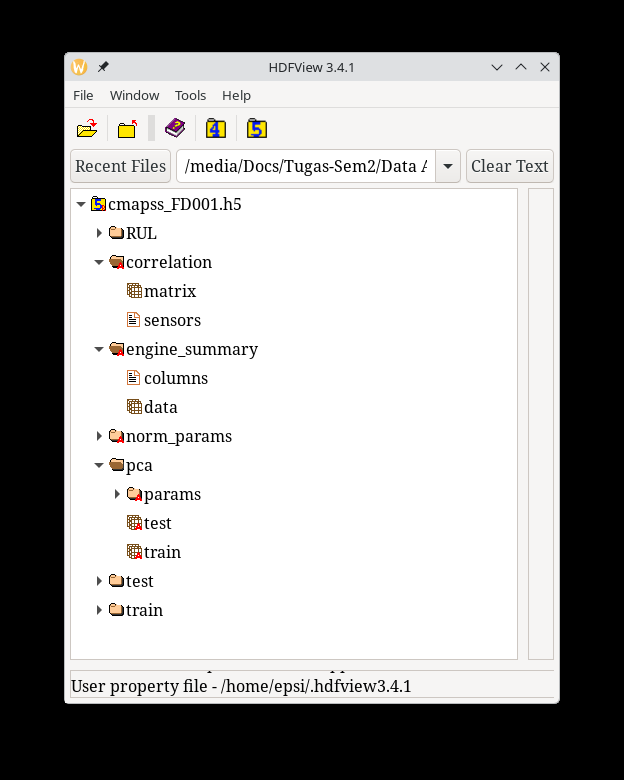
\includegraphics[width=0.38\textwidth]{images/hdf5-05-pca-01-main.png}
  \caption{Struktur HDF5 lengkap \texttt{cmapss\_FD001.h5} ditampilkan di HDFView}
  \label{fig:hdf5}
\end{figure}

Struktur HDF5 per file mencakup:
\texttt{/train/data} (32 kolom), \texttt{/train/data\_norm},
\texttt{/test/data} (29 kolom), \texttt{/test/data\_norm},
\texttt{/RUL/data}, \texttt{/norm\_params}, \texttt{/correlation},
\texttt{/engine\_summary}, dan \texttt{/pca}.

% ══════════════════════════════════════════════════════════════════════════════
\section{Pembersihan Data (\textit{Data Cleaning})}

\subsection{Identifikasi Sensor Konstan}

Tahap pembersihan data berfokus pada identifikasi sensor yang tidak membawa informasi
degradasi. Lima metode statistik digunakan secara bersamaan:

\begin{enumerate}[noitemsep]
  \item \textbf{Standar Deviasi} --- sensor dengan std $\approx 0$ bersifat konstan
  \item \textbf{Koefisien Variasi (CV)} --- cv $= \sigma/|\mu|$, nilai $< 0{,}001$ tidak informatif
  \item \textbf{Korelasi Pearson} --- mengukur hubungan linear dengan RUL
  \item \textbf{Korelasi Spearman} --- mengukur hubungan monoton dengan RUL
  \item \textbf{Mutual Information} --- menangkap hubungan non-linear dengan RUL
\end{enumerate}

\subsection{Hasil Analisis}

Sensor dengan std $= 0$ menghasilkan nilai Pearson dan Spearman tidak terdefinisi
(\texttt{NaN}) --- bukti matematis paling kuat untuk eliminasi. Tabel \ref{tab:drop}
merangkum sensor yang dieliminasi per sub-dataset.

\begin{table}[H]
\centering
\small
\caption{Sensor yang dieliminasi per sub-dataset (std $= 0$)}
\label{tab:drop}
\begin{tabular}{lcp{7cm}}
\toprule
Sub-dataset & Jumlah Dihapus & Sensor \\
\midrule
FD001 & 6 & T2, P2, epr, farB, Nf\_dmd, PCNfR\_dmd \\
FD002 & 0 & (tidak ada --- 6 kondisi operasi menyebabkan semua sensor bervariasi) \\
FD003 & 5 & T2, P2, farB, Nf\_dmd, PCNfR\_dmd \\
FD004 & 0 & (tidak ada) \\
\bottomrule
\end{tabular}
\end{table}

Perbedaan antara FD001/FD003 (1 kondisi) dan FD002/FD004 (6 kondisi) menunjukkan
bahwa sensor seperti T2 dan P2 bersifat konstan dalam satu kondisi operasi, namun
bervariasi antar kondisi. FD003 mempertahankan \texttt{epr} karena memiliki
std $= 0{,}0035$ (kecil namun bukan nol) akibat mode kerusakan HPC+Fan.

% ══════════════════════════════════════════════════════════════════════════════
\section{Normalisasi}

\subsection{Metode Z-Score Berbasis \textit{Healthy Cycles}}

Normalisasi menggunakan \textit{z-score} per kondisi operasi, dengan parameter
$\mu$ dan $\sigma$ dihitung hanya dari siklus \textit{healthy} (RUL\_raw $\geq 125$):

\begin{equation}
  z = \frac{x - \mu_c}{\sigma_c}
\end{equation}

di mana subscript $c$ menunjukkan kondisi operasi. Pendekatan ini memastikan
nilai $z = 0$ merepresentasikan kondisi mesin sehat, sehingga penyimpangan
dari nol mencerminkan degradasi.

Parameter normalisasi disimpan dalam \texttt{/norm\_params} dengan dimensi
$(n\_\text{kondisi} \times n\_\text{sensor})$: FD001/FD003 berukuran $(1, n_s)$
dan FD002/FD004 berukuran $(6, n_s)$.

Data \textit{test} dinormalisasi menggunakan parameter dari data \textit{train}
--- bukan parameter data \textit{test} itu sendiri --- untuk menghindari
\textit{data leakage}.

% ══════════════════════════════════════════════════════════════════════════════
\section{Seleksi Fitur}

\subsection{Korelasi Pearson}

Matriks korelasi Pearson dihitung dari \texttt{train\_normalized} untuk seluruh
21 sensor. Sensor konstan menghasilkan baris dan kolom \texttt{NaN}.

\begin{figure}[H]
  \centering
  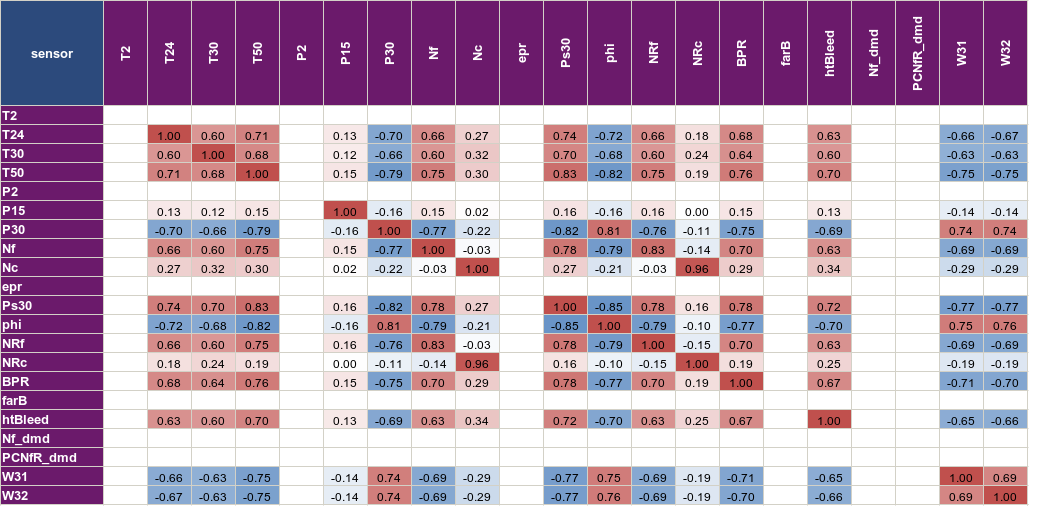
\includegraphics[width=0.75\textwidth]{images/spreadsheet-05-correlation-05-correlations.png}
  \caption{Matriks korelasi Pearson antar sensor (FD001) ---
    merah = korelasi positif kuat, biru = negatif kuat}
  \label{fig:corr}
\end{figure}

Pasangan sensor dengan $|r| > 0{,}90$ seperti Nf--NRf ($r = 0{,}83$) dan
Nc--NRc ($r = 0{,}96$) mengindikasikan redundansi informasi --- motivasi utama
penggunaan PCA.

\subsection{\textit{Principal Component Analysis} (PCA)}

PCA diterapkan pada data \textit{train\_normalized} untuk mereduksi dimensi.
Jumlah komponen dipilih berdasarkan \textbf{Opsi B}: pertahankan komponen dengan
varians individual $\geq 5\%$.

\begin{table}[H]
\centering
\small
\caption{Hasil PCA per sub-dataset --- jumlah komponen (Opsi B)}
\label{tab:pca}
\begin{tabular}{lcccc}
\toprule
Sub-dataset & Sensor & Komponen & Varians Kumulatif & Komponen Dominan \\
\midrule
FD001 & 15 & 2 & 82,9\% & PC1: speed sensors (52,4\%) \\
FD002 & 21 & 4 & 74,8\% & PC1: speed (41,6\%), PC3: epr (8,4\%) \\
FD003 & 16 & 3 & 87,8\% & PC1: speed (60,2\%) \\
FD004 & 21 & 3 & 77,5\% & PC1: speed (48,4\%) \\
\bottomrule
\end{tabular}
\end{table}

\begin{figure}[H]
  \centering
  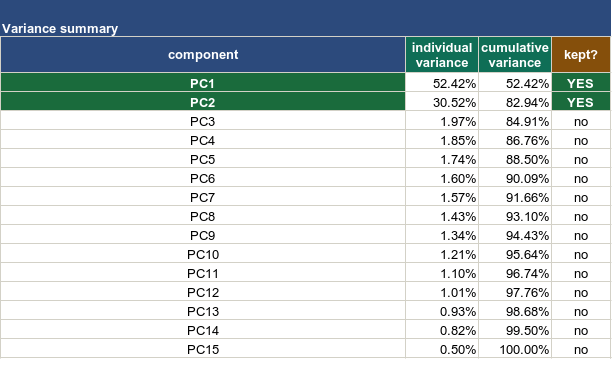
\includegraphics[width=0.75\textwidth]{images/spreadsheet-06-pca-11a-pca-params.png}
  \caption{Tabel varians PCA dan matriks \textit{eigenvectors} (FD002) ---
    PC3 didominasi oleh \texttt{epr} dengan \textit{loading} 0,94}
  \label{fig:pca_params}
\end{figure}

Temuan penting: pada FD002, PC3 hampir seluruhnya dijelaskan oleh \texttt{epr}
(\textit{loading} = 0,940). Sensor ini konstan di FD001 namun bervariasi antar
kondisi operasi di FD002, sehingga terisolasi menjadi komponen tersendiri.

% ══════════════════════════════════════════════════════════════════════════════
\section{Model \textit{Artificial Neural Network}}

\subsection{Arsitektur dan Konfigurasi}

Model \textit{Multilayer Perceptron} (MLP) dengan arsitektur:
\textit{input} $\rightarrow$ 64 $\rightarrow$ 32 $\rightarrow$ 1.
Fungsi aktivasi ReLU pada lapisan tersembunyi, output linear.

\begin{table}[H]
\centering
\small
\caption{Konfigurasi pelatihan model ANN}
\label{tab:ann_config}
\begin{tabular}{ll}
\toprule
Parameter & Nilai \\
\midrule
Arsitektur    & \textit{input} $\rightarrow$ 64 $\rightarrow$ 32 $\rightarrow$ 1 \\
Aktivasi      & ReLU (tersembunyi), Linear (output) \\
\textit{Loss} & MSE \\
Optimizer     & Adam, lr $= 10^{-3}$ \\
Epoch         & 500 \\
Batch size    & 512 \\
Target        & RUL\_capped (cap $= 125$ siklus) \\
\bottomrule
\end{tabular}
\end{table}

\subsection{Desain Eksperimen Benchmark}

Benchmark dirancang sebagai eksperimen 2-faktor:
\textbf{Faktor 1} --- sub-dataset (FD001--FD004);
\textbf{Faktor 2} --- tipe input (PCA vs. sensor ternormalisasi).
Total 8 model dilatih.

\begin{figure}[H]
  \centering
  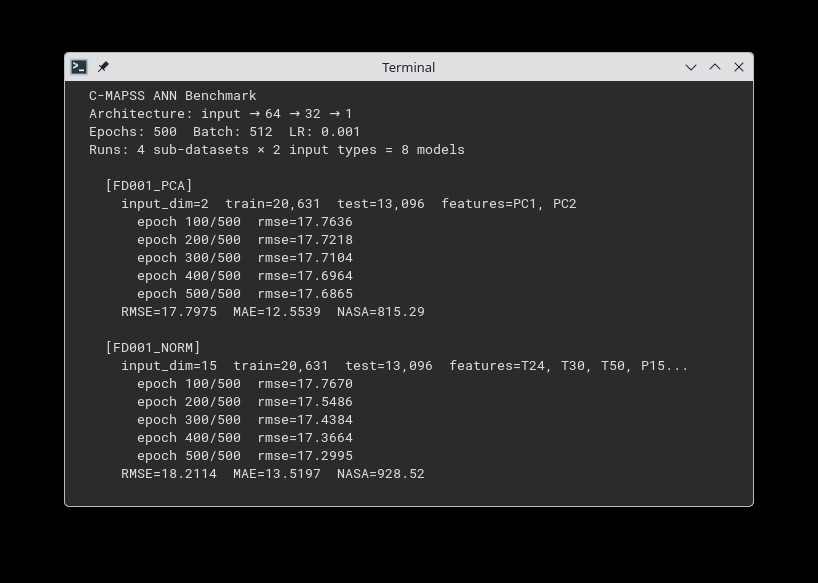
\includegraphics[width=0.80\textwidth]{images/python-08-build-ann-term-01.png}
  \caption{Output terminal pelatihan model ANN --- FD001 PCA dan NORM}
  \label{fig:ann_term}
\end{figure}

\subsection{Hasil Benchmark}

\begin{table}[H]
\centering
\small
\caption{Hasil benchmark 8 model --- RMSE, MAE, dan NASA Score}
\label{tab:benchmark}
\begin{tabular}{llcrrr}
\toprule
Sub-dataset & Input & Dim & RMSE & MAE & NASA Score \\
\midrule
FD001 & \textbf{PCA}  & 2  & \textbf{17,80} & \textbf{12,55} & \textbf{815} \\
FD001 & NORM & 15 & 18,21 & 13,52 & 929 \\
\midrule
FD002 & \textbf{PCA}  & 4  & \textbf{29,30} & \textbf{20,52} & 14.423 \\
FD002 & NORM & 21 & 29,45 & 20,73 & \textbf{12.990} \\
\midrule
FD003 & PCA  & 3  & 21,87 & 16,17 & 2.650 \\
FD003 & \textbf{NORM} & 16 & \textbf{20,16} & \textbf{15,28} & \textbf{1.783} \\
\midrule
FD004 & PCA  & 3  & 30,59 & 23,28 & 9.267 \\
FD004 & \textbf{NORM} & 21 & \textbf{29,68} & \textbf{22,38} & \textbf{7.157} \\
\bottomrule
\end{tabular}
\end{table}

\begin{figure}[H]
  \centering
  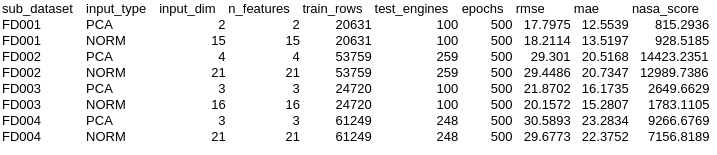
\includegraphics[width=0.70\textwidth]{images/ann-06-00-summary.png}
  \caption{File \texttt{summary.csv} hasil benchmark dibuka di LibreOffice Calc}
  \label{fig:summary}
\end{figure}

\subsection{Analisis Hasil}

\textbf{Pengaruh Faktor 1 (sub-dataset):}
Kompleksitas kondisi operasi menjadi faktor dominan.
Sub-dataset dengan 1 kondisi (FD001, FD003) menghasilkan RMSE $\approx 18$--$22$,
sedangkan sub-dataset dengan 6 kondisi (FD002, FD004) menghasilkan RMSE $\approx 29$--$31$
--- peningkatan sekitar 60\%.

\textbf{Pengaruh Faktor 2 (tipe input):}
\begin{itemize}[noitemsep]
  \item \textbf{1 kondisi operasi}: PCA mengungguli NORM pada FD001 dan FD002 (berdasarkan RMSE).
    Kompresi PCA menghilangkan \textit{noise} secara efektif ketika masalah sederhana.
  \item \textbf{6 kondisi operasi}: NORM mengungguli PCA pada FD003 dan FD004.
    Sensor penuh mempertahankan informasi spesifik kondisi yang hilang dalam kompresi PCA.
\end{itemize}

\textbf{NASA Score FD002 yang tinggi} (14.423 vs. $\sim$815 untuk FD001)
mengindikasikan banyak prediksi \textit{late} --- model cenderung melebih-estimasi RUL
pada data dengan 6 kondisi operasi yang kompleks.

% ══════════════════════════════════════════════════════════════════════════════
\section{Analisis Garson}

\subsection{Algoritma Garson}

Algoritma Garson \cite{garson1991} menghitung kepentingan relatif setiap fitur input
berdasarkan bobot jaringan yang telah dilatih. Untuk arsitektur dua lapisan
tersembunyi ($W_1$, $W_2$, $W_3$):

\begin{equation}
  q_1[i,j] = \frac{|W_1[j,i]|}{\sum_k |W_1[j,k]|}, \quad
  q_2[j,m] = \frac{|W_2[m,j]|}{\sum_k |W_2[m,k]|}
\end{equation}

\begin{equation}
  r[i,m] = \sum_j q_1[i,j] \cdot q_2[j,m], \quad
  s[i]   = \sum_m r[i,m] \cdot |W_3[m]|, \quad
  \text{importance}[i] = \frac{s[i]}{\sum_k s[k]}
\end{equation}

\subsection{Hasil Analisis Garson}

\begin{figure}[H]
  \centering
  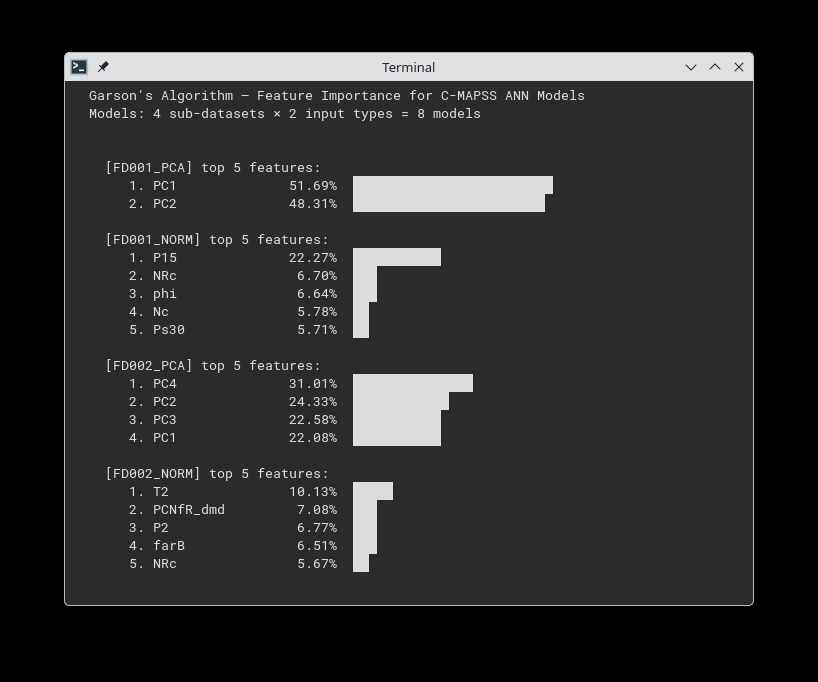
\includegraphics[width=0.75\textwidth]{images/python-09-garson-term-01.png}
  \caption{Output terminal algoritma Garson --- top 5 fitur per model}
  \label{fig:garson_term}
\end{figure}

\begin{table}[H]
\centering
\small
\caption{Lima fitur terpenting per model (algoritma Garson)}
\label{tab:garson}
\begin{tabular}{llp{9cm}}
\toprule
Model & Fitur \#1 & Top 5 Fitur \\
\midrule
FD001\_PCA  & PC1 (51,7\%) & PC1 51,7\% --- PC2 48,3\% \\
FD001\_NORM & P15 (22,3\%) & P15 22,3\% --- NRc 6,7\% --- phi 6,6\% --- Nc 5,8\% --- Ps30 5,7\% \\
FD002\_PCA  & PC4 (31,0\%) & PC4 31,0\% --- PC2 24,3\% --- PC3 22,6\% --- PC1 22,1\% \\
FD002\_NORM & T2  (10,1\%) & T2 10,1\% --- PCNfR\_dmd 7,1\% --- P2 6,8\% --- farB 6,5\% --- NRc 5,7\% \\
FD003\_PCA  & PC2 (37,9\%) & PC2 37,9\% --- PC3 35,7\% --- PC1 26,5\% \\
FD003\_NORM & P15 (14,7\%) & P15 14,7\% --- epr 8,0\% --- phi 6,8\% --- P30 6,4\% --- NRc 6,3\% \\
FD004\_PCA  & PC2 (42,3\%) & PC2 42,3\% --- PC3 31,8\% --- PC1 26,0\% \\
FD004\_NORM & T2  (9,9\%)  & T2 9,9\% --- P2 9,3\% --- P15 8,4\% --- Ps30 5,5\% --- phi 5,2\% \\
\bottomrule
\end{tabular}
\end{table}

\subsection{Perbandingan Tiga Metode Seleksi Fitur}

\begin{table}[H]
\centering
\small
\caption{Perbandingan kepentingan sensor berdasarkan tiga metode (FD001)}
\label{tab:three_method}
\begin{tabular}{lcccp{4cm}}
\toprule
Sensor & Pearson vs RUL & PCA Loading & Garson (ANN) & Interpretasi \\
\midrule
Ps30 & $-0{,}70$ & tinggi   & sedang & Konsisten --- penting \\
T50  & $-0{,}68$ & tinggi   & sedang & Konsisten --- penting \\
P30  & $+0{,}66$ & tinggi   & sedang & Konsisten --- penting \\
P15  & $-0{,}13$ & rendah   & \textbf{tinggi} & Perbedaan --- ANN menemukan sinyal non-linear \\
NRf  & $-0{,}56$ & sedang   & rendah & Sebagian konsisten \\
\bottomrule
\end{tabular}
\end{table}

Temuan penting: sensor \textbf{P15} memiliki korelasi Pearson rendah ($-0{,}13$)
dan kontribusi PCA rendah, namun Garson menetapkannya sebagai fitur terpenting
(22,3\%) pada model FD001\_NORM. Hal ini mengindikasikan bahwa ANN mampu
mengeksploitasi hubungan non-linear yang tidak terdeteksi oleh Pearson dan PCA.

Pada FD002\_NORM, sensor \textbf{T2, P2, PCNfR\_dmd} dan \textbf{farB} ---
yang dieliminasi dari FD001 karena std $= 0$ --- justru muncul sebagai fitur
terpenting. Ini mengkonfirmasi bahwa eliminasi sensor harus dilakukan per
sub-dataset, bukan secara universal.

% ══════════════════════════════════════════════════════════════════════════════
\section{Kesimpulan}

Pipeline analitik lengkap telah berhasil diimplementasikan untuk prediksi RUL
mesin turbofan menggunakan dataset C-MAPSS, dengan temuan utama sebagai berikut:

\begin{enumerate}[noitemsep]
  \item \textbf{Kompleksitas kondisi operasi} adalah faktor dominan yang memengaruhi
    akurasi prediksi. Sub-dataset dengan 6 kondisi (FD002, FD004) menghasilkan RMSE
    $\approx 29$--$31$ dibandingkan $18$--$22$ untuk sub-dataset 1 kondisi.

  \item \textbf{Tipe input optimal bergantung pada kompleksitas dataset}:
    PCA lebih baik untuk dataset sederhana (1 kondisi), sensor penuh lebih baik
    untuk dataset kompleks (6 kondisi). Ini konsisten dengan teori --- PCA
    membuang 17\% varians yang justru relevan ketika sinyal degradasi tersebar
    di banyak kondisi.

  \item \textbf{Algoritma Garson} mengungkap hubungan non-linear yang tidak
    terdeteksi oleh Pearson dan PCA --- khususnya sensor P15 yang rendah secara
    linear namun tinggi secara kepentingan ANN.

  \item \textbf{Eliminasi sensor harus bersifat per sub-dataset}: sensor konstan
    di FD001 (T2, P2) menjadi fitur terpenting di FD002, karena variasi antar
    kondisi operasi mengandung informasi degradasi.
\end{enumerate}

% ── References ────────────────────────────────────────────────────────────────
\begin{thebibliography}{9}

\bibitem{saxena2008}
  A. Saxena, K. Goebel, D. Simon, N. Eklund,
  ``Damage Propagation Modeling for Aircraft Engine Run-to-Failure Simulation,''
  \textit{Proceedings of the 1st International Conference on Prognostics and
  Health Management (PHM08)}, Denver, CO, 2008.

\bibitem{garson1991}
  G.D. Garson,
  ``Interpreting Neural Network Connection Weights,''
  \textit{AI Expert}, vol.~6, no.~4, pp.~46--51, 1991.

\end{thebibliography}

\end{document}
